\documentclass[10pt,prd,nofootinbib,superscriptaddress,twocolumn]{revtex4-2}
\pdfoutput=1


%%%%%%%%%%%%% Packages %%%%%%%%%%%%%
% general
\usepackage[utf8]{inputenc}
\usepackage{geometry}
\geometry{
	a4paper,
	total={170mm,257mm},
	left=20mm,
	top=20mm,
}

% math
\usepackage{mathtools}
\usepackage{amsfonts}
\usepackage{dsfont}
\usepackage{mathrsfs}
\usepackage{bbm}
\usepackage[normalem]{ulem}
\usepackage{slashed}
\usepackage{tensor}

\usepackage{pifont}
\newcommand{\xmark}{\ding{55}}

% graphics and colours
\usepackage{graphicx}
\usepackage{array}

% floats
\usepackage{placeins}
\usepackage{makecell}
\usepackage{float}

% units and refs
\usepackage{xspace}
\usepackage{xfrac}
\usepackage{hyperref}
\usepackage[nameinlink]{cleveref}
\usepackage{appendix}
\usepackage{units}

% text formatting
% Get rid of single letters at the end of lines and repeated hyphenation
\usepackage[hyphenation]{impnattypo}
% Get rid of widows and orphans
\usepackage[all]{nowidow}
\usepackage{microtype}

% other
\usepackage{xifthen}
\usepackage{booktabs}
\usepackage{multirow}
\usepackage[dvipsnames]{xcolor}
\hypersetup{
	colorlinks,
	linkcolor={red!75!black},
	citecolor={blue!75!black},
	urlcolor={blue!75!black},
	pdftitle={FunKit: A toolkit for functional approaches},
	pdfauthor={Sattler},
}
\usepackage{enumerate}


\newcommand{\innerproduct}[2]{\left\langle #1, #2 \right\rangle}
\newcommand{\imag}{\text{i}}
\newcommand{\norm}[1]{\left\lVert#1\right\rVert}

%%%%%%%%%%%%% Comments %%%%%%%%%%%%%
\newcommand{\commentFS}[1]{\textcolor{blue}{[\textbf{FS:} #1]}}
\newcommand{\cJMP}[1]{\textcolor{blue}{\textbf{Jan: #1}}}

%%%%%%%%%%%%% Mathematica code %%%%%%%%%%%%%
\usepackage{mmacells}
\mmaDefineMathReplacement[≤]{<=}{\leq}
\mmaDefineMathReplacement[≥]{>=}{\geq}
\mmaDefineMathReplacement[≠]{!=}{\neq}
\mmaDefineMathReplacement[→]{->}{\to}[2]
\mmaDefineMathReplacement[⧴]{:>}{:\hspace{-.2em}\to}[2]
\mmaDefineMathReplacement{∉}{\notin}
\mmaDefineMathReplacement{∞}{\infty}
\mmaDefineMathReplacement{𝕕}{\mathbbm{d}}
\mmaSet{
	leftmargin=3.0em,
	morefv={gobble=0},
	linklocaluri=mma/symbol/definition:#1,
	morecellgraphics={yoffset=0ex},
	fv={formatcom*=\small\normalfont\ttfamily},
	labelsep=0.em,
}

%%%%%%%%%%%%%%%%%%%%%%%%%%%%%%%%%%%%%%%%%%%

\usepackage{listings}
\definecolor{backcolor}{rgb}{0.99,0.98,0.98}
\definecolor{string-color}{rgb}{0.3333, 0.5254, 0.345}
\definecolor{darkgrey}{rgb}{0.0627, 0.07, 0.082}
\definecolor{darkred}{rgb}{0.3, 0.05, 0.05}
\definecolor{codeblue}{rgb}{0.2,0.35,0.75}
\definecolor{codepurple}{rgb}{0.38,0.1,0.52}
\definecolor{codegray}{rgb}{0.5,0.5,0.5}
\definecolor{codegreen}{rgb}{0.05,0.3,0.05}
\definecolor{codered}{rgb}{0.6,0.2,0.1}
\definecolor{backgroundColour}{rgb}{0.99,0.99,0.98}
\lstdefinestyle{myStyle}{
	language = C++,
	basicstyle = {\ttfamily \small \color{darkgrey}},
	backgroundcolor = {\color{backcolor}},
	commentstyle=\color{codegreen},
	stringstyle = {\color{string-color}},
	keywordstyle = {\color{codeblue}},
	keywordstyle = [2]{\color{codepurple}},
	keywordstyle = [3]{\color{codered}},
	keywordstyle = [4]{\color{codegray}},
	keywordstyle = [5]{\color{codegreen}},
	otherkeywords = {<, >, :, ::, DiFfRG, constexpr, uint, size_t, &, get, vector, array, Tensor, Scalar, FunctionND},
	morekeywords = [2]{AbstractModel, FEFunctionDescriptor, VariableDescriptor, ExtractorDescriptor, ComponentDescriptor
		TimeStepperSUNDIALS_IDA, UMFPack, Point, real, AD, NoJacobians, FE_AD,LLFFlux,FlowBoundaries
	},
	morekeywords = [3]{DiFfRG, CG, DG, dDG, LDG, def, Variables, dealii, std, autodiff},
	morekeywords = [4]{<, >, :, ::, ;, &},
	morekeywords = [5]{},
	breakatwhitespace=false,
	breaklines=true,
	captionpos=b,
	keepspaces=true,
	numbers=none,
	numbersep=5pt,
	numberstyle=\scriptsize\color{darkred},
	showspaces=false,
	showstringspaces=false,
	showtabs=false,
	tabsize=2
}
\lstdefinestyle{genStyle}{
	basicstyle = {\ttfamily \small \color{darkgrey}},
	backgroundcolor = {\color{backcolor}},
	commentstyle=\color{codegreen},
	stringstyle = {\color{string-color}},
	keywordstyle = {\color{codeblue}},
	breakatwhitespace=false,
	breaklines=true,
	captionpos=b,
	keepspaces=true,
	numbers=none,
	numbersep=5pt,
	numberstyle=\scriptsize\color{darkred},
	showspaces=false,
	showstringspaces=false,
	showtabs=false,
	tabsize=2
}
\lstset{style=genStyle}
\lstdefinelanguage{CMake}{%
	morekeywords={if, else, endif, project, cmake_minimum_required, set, find_package, add_executable},%
	sensitive=false,%
	morecomment=[l]{\#},%
	morecomment=[s]{/*}{*/},%
	morestring=[b]",%
	otherkeywords={add_flows, setup_application},%
	keywordstyle = [2]{\color{codepurple}},
	morekeywords = [2]{REQUIRED, HINTS, VERSION, SYSTEM},
}
\lstdefinelanguage{Bash}{%
	morekeywords={if, else, fi, mkdir, cd, cmake, bash, git},%
	sensitive=false,%
	morecomment=[l]{\#},%
	morecomment=[s]{/*}{*/},%
	morestring=[b]",%
	keywordstyle = {\color{codeblue}},
	keywordstyle = [2]{\color{codepurple}},
	morekeywords = [2]{$, /, ..},
}


%%%%%%%%%%%%% Inline code shortcuts %%%%%%%%%%%%%
\newcommand{\cpp}{\lstinline[language=C++,style=myStyle]}
\newcommand{\cmake}{\lstinline[language=CMake]}
\newcommand{\mathem}{\mmaInlineCell{Code}}
\newcommand{\bash}{\lstinline[language=Bash]}

%%%%%%%%%%%%%%%%%%% MARCROS %%%%%%%%%%%%%
\newcommand{\LEGO}{LEGO\textsuperscript{\textregistered}}
\newcommand{\FunKit}{\texttt{FunKit}\xspace}
\newcommand{\FEDeriK}{\texttt{FEDeriK}\xspace}
\newcommand{\DiANE}{\texttt{DiANE}\xspace}
\newcommand{\AnSEL}{\texttt{AnSEL}\xspace}
\newcommand{\tinytext}[1]{\text{\tiny{#1}}}
\newcommand{\TensorBases}{\texttt{TensorBases}\xspace}

%%%%%%%%%%%%% Graphic paths %%%%%%%%%%%%%
\graphicspath{{./figures/}}

\renewcommand{\floatpagefraction}{.8}


%%%%%%%%%%%%% Title and hypersetup %%%%%%%%%%%%%
\newcommand{\gettitle}{FunKit: A toolkit for functional approaches}

\newcommand{\getHeidelbergAffiliation}{\affiliation{Institut f{\"u}r Theoretische Physik, Universit{\"a}t Heidelberg, Philosophenweg 16, 69120 Heidelberg, Germany}}
\newcommand{\getBielefeldAffiliation}{\affiliation{Fakult{\"a}t f{\"u}r Physik, Universit{\"a}t Bielefeld, D-33615 Bielefeld, Germany}}
\newcommand{\getDarmstadtAffiliation}{\affiliation{Institut f\"ur Kernphysik (Theoriezentrum), Technische Universit\"at Darmstadt, 64289 Darmstadt, Germany}}
\newcommand{\getEMMIAffiliation}{\affiliation{ExtreMe Matter Institute EMMI, GSI, Planckstr. 1, 64291 Darmstadt, Germany}}

\newcommand{\orcid}[1]{\href{https://orcid.org/#1}{
\includegraphics[height=1.9ex,width=1.9ex]{figures/orcid.png}}}

\begin{document}

\title{\gettitle}
\author{Franz R. Sattler \orcid{0000-0003-1744-9456}\,}\thanks{\url{sattler@thphys.uni-heidelberg.de}}
\getHeidelbergAffiliation\getBielefeldAffiliation
%\author{Jan M. Pawlowski \orcid{0000-0003-0003-7180}\,}
%\getHeidelbergAffiliation
%\getEMMIAffiliation

\begin{abstract}

We give tool to compute cross-section
\end{abstract}

\maketitle

%%%%%%%%%%%%%%%%%%%%%%%%%%%%%%
\section{Introduction}
\label{sec:Introduction}

\texttt{DoFun} \cite{Huber:2019dkb} and \texttt{QMeS} \cite{Pawlowski:2021tkk}

\TensorBases \cite{Braun:2025gvq}


%%%%%%%%%%%%%%%%%%%%%%%%%%%%%%
\section{Deriving functional equations}
\label{sec:FEDeriK}

\FEDeriK, the {\textbf{F}unctional \textbf{E}quation \textbf{Deri}vation \textbf{K}it} is the core module of \FunKit, providing all the logic to derive functional equations. In particular, it provides the base syntax for the description of functional equations, gives facilities to perform functional derivatives and series expansions of derivative operators and fields.


\AnSEL, \textbf{An}alysis and \textbf{S}implification of \textbf{E}quations with \textbf{L}oops

In \Cref{sec:FEDeriK_notation} we briefly explain both the notation in \texttt{Mathematica} and basic usage of the module. Following this, we explain the internal set of rules used by \FEDeriK in \Cref{sec:FEDeriK_rules} and some algorithmic details in \Cref{sec:FEDeriK_algorithm}.

%%%%%%%%%%%%%%%%%%%%
\subsection{Notation \& usage}
\label{sec:FEDeriK_notation}

\subsubsection{Syntax}

A single term in a functional equation is described using the \mathem{\mmaDef{FTerm}} tag, which encloses a list of factors. For example, the Wetterich equation $\frac{1}{2}G^{ab}\partial_tR_{ab}$ can be written as the term
%

\begin{mmaCell}{Input}
 wEq = \mmaDef{FTerm}[1/2,
   \mmaDef{Propagator}[\{\mmaDef{AnyField},\mmaDef{AnyField}\},\{a,b\}],
   \mmaDef{Rdot}[\{\mmaDef{AnyField},\mmaDef{AnyField}\},\{-a,-b\}]]
\end{mmaCell}
%
Here, we have also used \FEDeriK's common notation for any indexed object. \FEDeriK knows, by default, the following indexed objects:
%
\begin{mmaCell}{Input}
 \mmaDef{ShowIndexedObjects}[]
\end{mmaCell}
\begin{mmaCell}{Output}
 ABasis
 GammaN
 Propagator
 Rdot
 S
 VBasis
 \({\gamma}\)
\end{mmaCell}
%
Lowered superindices are indicated by a minus sign. As an example, the correlation function $\Gamma_{a\,b\,A^c}^{\phantom{a\,b\,A^c}\bar{c}^d}$, with the fields of $a$ and $b$ undetermined, may be expressed~as
%
\begin{mmaCell}{Input}
 \mmaDef{GammaN}[\{\mmaDef{AnyField},\mmaDef{AnyField},A,cb\},
   \{-a,-b,-c,d\}]
\end{mmaCell}
%
The tag \mathem{\mmaDef{AnyField}} stands in for arbitrary fields, which can be expanded into explicit fields later on.

Sums of functional equations are represented using the \mathem{\mmaDef{FEx}} tag. As an example, we take the generalised flow equation
%
\begin{equation}
	\partial_t \Gamma = -\dot\Phi^a\Gamma_a + \frac{1}{2}G^{ac}(\gamma_c^{\phantom{c}b}\partial_t + \frac{\delta\dot{\Phi}^b}{\delta\Phi^c}){R}_{ab}
	\,.
\end{equation}
%
For conciseness, we redefine $(\gamma_b^{\phantom{b}c}\partial_t + \frac{\delta\dot{\Phi}^c}{\delta\Phi^b}){R}_{ac} \to \partial_t R_{ab}$ and shorten the equation to 
$\partial_t \Gamma = -\dot\Phi^a\Gamma_a + \frac{1}{2}G^{ab}\partial_t{R}_{ab}$.
Hence, it can be expressed~with
%
\begin{mmaCell}{Input}
 \mmaDef{AddCorrelationFunction}[Phidot,1];
 \mmaDef{SetUnorderedIndices}[Phidot];
 \mmaDef{FEx}[
   \mmaDef{FTerm}[-Phidot[\{\mmaDef{AnyField}\},\{a\}], 
     \mmaDef{GammaN}[\{\mmaDef{AnyField}\},\{-a\}]]
   \mmaDef{FTerm}[1/2, 
     \mmaDef{Propagator}[\{\mmaDef{AnyField},\mmaDef{AnyField}\},\{a,b\}],
     \mmaDef{Rdot}[\{\mmaDef{AnyField},\mmaDef{AnyField}\},\{-a,-b\}]]
  ];
\end{mmaCell}
%
In the above, we have also informed \FEDeriK about a user-defined correlation function, \mathem{Phidot} $\equiv \dot{\Phi}$, and told it to never change the position of the last index (i.e. the superindex specifying $\Phi$ itself).
\FEDeriK will automatically treat \mathem{Phidot} as a field-dependent function and take into account derivatives thereof.

\mathem{\mmaDef{FEx}} and \mathem{\mmaDef{FTerm}} have some internal rules to automatically move numeric values to the first factor in any \mathem{\mmaDef{FTerm}} and expand any appearance of sums to the enclosing \mathem{\mmaDef{FEx}}. This behaviour can be seen, e.g. in
%
\begin{mmaCell}{Input}
 \mmaDef{FEx}[\mmaDef{FTerm}[a+b,2,4c,\mmaDef{FEx}[\mmaDef{FTerm}[d+e]]]]
\end{mmaCell}
\begin{mmaCell}{Output}
 \mmaDef{FEx}[\mmaDef{FTerm}[8,a,c,d], \mmaDef{FTerm}[8,a,c,e],
   \mmaDef{FTerm}[8,b,c,d], \mmaDef{FTerm}[8,b,c,e]]
\end{mmaCell}
%
\mathem{\mmaDef{FEx}} and \mathem{\mmaDef{FTerm}} can be multiplied using non-commutative multiplication, 
%
\begin{mmaCell}{Input}
 \mmaDef{FEx}[\mmaDef{FTerm}[a+b,2]]**\mmaDef{FEx}[\mmaDef{FTerm}[d+e]]
\end{mmaCell}
\begin{mmaCell}{Output}
 \mmaDef{FEx}[\mmaDef{FTerm}[2,a,d], \mmaDef{FTerm}[2,a,e],
   \mmaDef{FTerm}[2,b,d], \mmaDef{FTerm}[2,b,e]]
\end{mmaCell}
%
Normal multiplication immediately yields an error, as the factors in a given \mathem{\mmaDef{FTerm}} are not necessarily commuting.

\subsubsection{Field setup}

Most functions defined by \FunKit require the specification of a \textit{setup}. A setup is given by an \mathem{\mmaDef{Assocation}} with the mandatory key \mathem{"FieldSpace"} and further optional keys, which we will specify below.

The field content of the theory is specified using another \mathem{\mmaDef{Assocation}} with two entries, \mathem{"cField"}, and \mathem{"Grassmann"}. The value of these entries is a list of all fields occurring in the theory. For example, the fields of a gauge-fixed Yang-Mills theory can be given as
%
\begin{mmaCell}{Input}
 fields = <|
   "cField" -> \{A[p,\{v,c\}]\},
   "Grassmann" -> \{\{cb[p,\{c\}], c[p,\{c\}]\}\}
  |>;
\end{mmaCell}
%
The gauge field \mathem{A} is a commuting field and has no partner field. In contrast, there are ghosts and anti-ghosts \mathem{cb}, \mathem{c}, hence they are specified as a pair in a nested list.
Fields are always specified together with their full index structure. A momentum variable is obligatory, i.e. a purely scalar field space could be specified as
%
\begin{mmaCell}{Input}
 fieldsPhi = <|
   "cField" -> \{\(\pmb{\phi}\)[p]\},
   "Grassmann" -> \{\}
  |>;
\end{mmaCell}
%
In the above case of Yang-Mills theory, all fields have additional group structure. These indices must be fully specified with a second, optional list in the argument of the field.

The resulting setup is then given as
%
\begin{mmaCell}{Input}
 setup = <|
   "FieldSpace" -> \mmaDef{fields}
  |>;
\end{mmaCell}
%

\subsection{Deriving diagrams}

With the \mathem{\mmaDef{setup}} defined, one can immediately start deriving diagrams.
Above, we have defined the Wetterich equation as \mathem{\mmaDef{wEq}}. We can obtain the RG-flow of the gluon two-point function using
%
\begin{mmaCell}{Input}
 \mmaDef{TakeDerivatives}[\mmaDef{wEq}, \{A[i1], A[i2]\}];
\end{mmaCell}
%
This will yield a rather large expression, which we can visualise using the \mathem{\mmaDef{FPrint}} and \mathem{\mmaDef{FPlot}} commands, which will be explained in more detail within \Cref{sec:DiANE}.
%
\begin{widetext}
\vspace{-2pt}
%\hspace{40pt}
\begin{minipage}{0.7\linewidth}
\begin{mmaCell}{Input}
 \mmaDef{TakeDerivatives}[\mmaDef{wEq}, \{A[i1], A[i2]\}]//\mmaDef{FPrint}//\mmaDef{FPlot};
\end{mmaCell}
\vspace{-2.5ex}
\begin{equation*}
	\put(-132,0){\footnotesize
		$
		\begin{aligned}&
			(-1)^{A^{i_1}\text{a}}\,(-1)^{A^{i_2}\text{a}}\,(-1)^{\text{c}\text{c}}\,(-1)^{\text{e}\text{e}}\,G^{\text{a}\text{b}}\,\Gamma_{\text{b}A^{i_2}\text{c}}\,G^{\text{c}\text{d}}\,\Gamma_{\text{d}A^{i_1}\text{e}}\,G^{\text{e}\text{f}}\,\partial_t R_{\text{a}\text{f}}
			\\ &\,+\,
			(-\frac{1}{2}\,(-1)^{A^{i_1}\text{a}}\,(-1)^{\text{c}\text{c}}\,G^{\text{a}\text{b}}\,(-1)^{A^{i_2}\text{a}}\,(-1)^{A^{i_2}\text{b}}\,\Gamma_{A^{i_2}\text{b}A^{i_1}\text{c}}\,G^{\text{c}\text{d}}\,\partial_t R_{\text{a}\text{d}})
		\end{aligned}
		$
	}
	\put(-132,-83){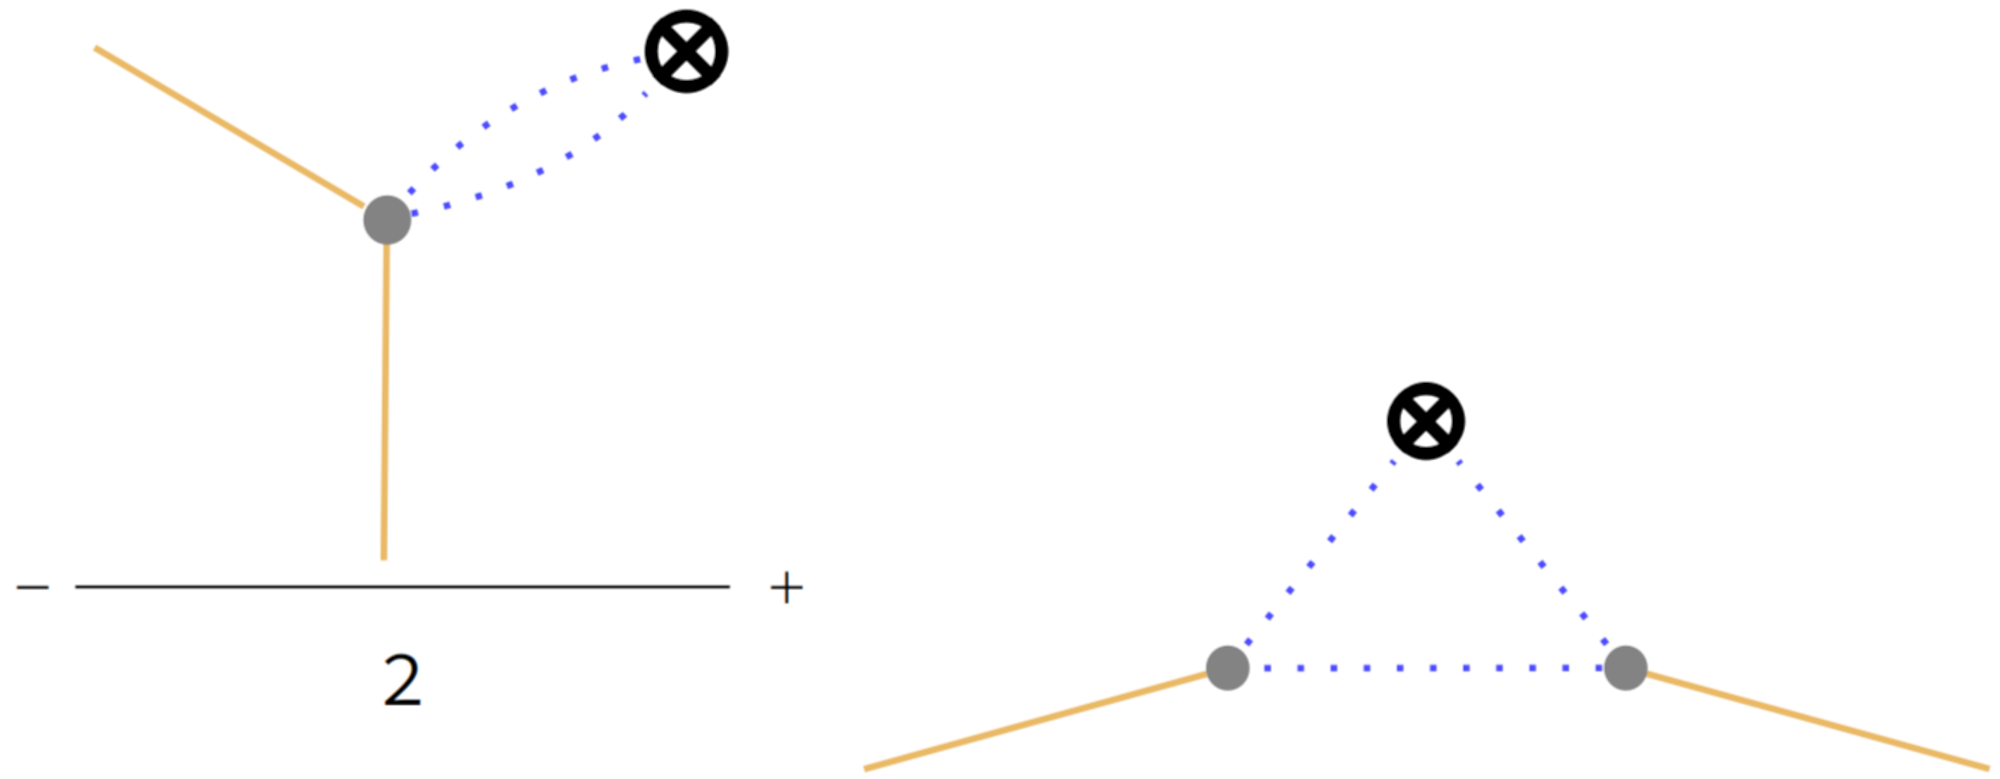
\includegraphics[width=0.48\linewidth]{Mathematica_Gluon2P_1.png}}
\end{equation*}
\end{minipage}
\end{widetext}
%
\FunKit has automatically simplified the diagrams resulting from the derivation. We can also do the above in a more manual manner by explicitly specifying derivative operators and resolving them. Any functional derivative is specified as an operator \mathem{\mmaDef{FDOp}} acting on everything after it. To resolve derivatives, \FunKit provides the functions \mathem{\mmaDef{ResolveFDOp}} to resolve the right-most \mathem{\mmaDef{FDOp}} in an expression, and \mathem{\mmaDef{ResolveDerivatives}} to fully resolve all derivatives. Explicitly, we can write the above also as
%
\begin{widetext}
%\vspace{-2pt}
%\hspace{40pt}
\begin{minipage}{0.5\linewidth}
\begin{mmaCell}{Input}
 \mmaDef{ResolveFDOp}[
   \mmaDef{ResolveFDOp}[
     \mmaDef{F}[\mmaDef{FDOp}@A[i1], \mmaDef{FDOp}@A[i2], \mmaDef{wEq}]
    ]
  ]//\mmaDef{FPrint}//\mmaDef{FPlot};
\end{mmaCell}
\vspace{-2.5ex}
\begin{equation*}
		\put(-82,0){\footnotesize
			$
		\begin{aligned}&
			\frac{1}{2}\,(-1)^{A^{i_1}\text{a}}\,(-1)^
			{A^{i_2}\text{a}}\,(-1)^{\text{c}\text{c}}
			\,(-1)^{\text{e}\text{e}}\,G^{\text{a}\text{b}}\,\Gamma_{\text{b}A^{i_1}\text{c}}\,G
			^{\text{c}\text{d}}\,\Gamma_{\text{d}A^{i_
					2}\text{e}}\,G^{\text{e}\text{f}}\,\partial_t R_{\text{a}\text{f}}
			\\ &\,+\,
			(-\frac{1}{2}\,(-1)^{A^{i_2}\text{a}}\,(-1
			)^{\text{c}\text{c}}\,G^{\text{a}\text{b}}
			\,(-1)^{A^{i_1}\text{a}}\,(-1)^{A^{i_1}\text{b}}\,\Gamma_{A^{i_1}\text{b}A^{i_2}\text{c}}\,G^{\text{c}\text{d}}\,\partial_t
			R_{\text{a}\text{d}})
			\\ &\,+\,
			\frac{1}{2}\,(-1)^{A^{i_2}\text{a}}\,(-1)^
			{\text{c}\text{c}}\,G^{\text{a}\text{b}}\,
			\Gamma_{\text{b}A^{i_2}\text{c}}\,(-1)^{A^
				{i_1}\text{a}}\,(-1)^{\text{e}\text{e}}\,G
			^{\text{c}\text{d}}\,\Gamma_{\text{d}A^{i_1}\text{e}}\,G^{\text{e}\text{f}}\,\partial_t R_{\text{a}\text{f}}
		\end{aligned}
			$
		}
		\put(-82,-88){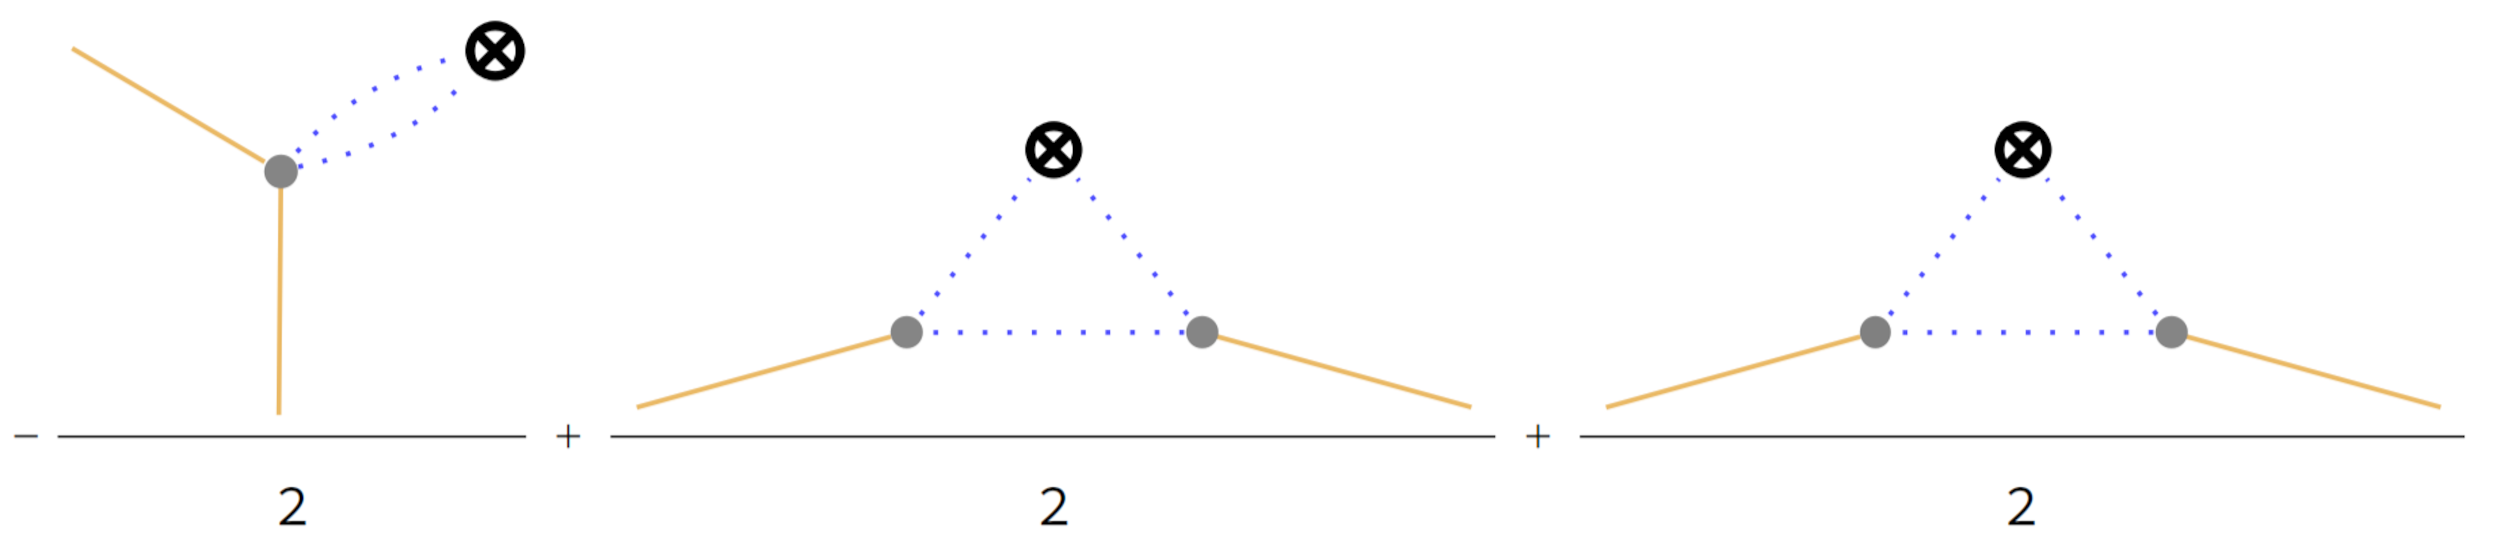
\includegraphics[width=1.1\linewidth]{Mathematica_Gluon2P_2.png}}
\end{equation*}
\end{minipage}
\end{widetext}
%
In the above, we have used the shorthand \mathem{\mmaDef{F}[...]}, which is replaced by \mathem{\mmaDef{FEx}[\mmaDef{FTerm}[...]]}. The result of resolving the derivative operators has not been automatically simplified. This can be done using \mathem{\mmaDef{FSimplify}}, i.e.
%
\begin{mmaCell}{Input}
 \mmaDef{ResolveFDOp}[
   \mmaDef{ResolveFDOp}[
     \mmaDef{F}[\mmaDef{FDOp}@A[i1], \mmaDef{FDOp}@A[i2], \mmaDef{wEq}]
    ]
  ]//\mmaDef{FSimplify}//\mmaDef{FPrint}//\mmaDef{FPlot};
\end{mmaCell}
%
which yields precisely the same output as when using \mathem{\mmaDef{TakeDerivatives}} or \mathem{\mmaDef{ResolveDerivatives}}, both of which invoke the simplification step automatically.


%%%%%%%%%%%%%%%%%%%%%%%%%%%%%%%%%%%%%%%%
\subsection{Truncating the output}

The above equation still contains undetermined fields, which are expressed by superindices without fields in the equations and by dotted blue lines in the diagrams.
To insert explicit fields, we first have to supply a truncation. this is done by creating a list for every correlation function or indexed object which contains all field combinations to be taken into account:
%
\begin{mmaCell}{Input}
 truncation = <|
   \mmaDef{GammaN} -> \{\{A,A\},\{A,A,A\},\{A,A,A,A\},
              \{A,cb,c\},\{cb, c\}\},
   \mmaDef{Propagator} -> \{\{A,A\},\{cb, c\}\},
   \mmaDef{Rdot} -> \{\{A,A\},\{cb, c\}\},
   \mmaDef{S} -> \{\{A,A\},\{A,A,A\},\{A,A,A,A\},
         \{cb,c\},\{cb,c,A\}\},
   \mmaDef{Field} -> \{\{\}\}
 |>;
\end{mmaCell}
%
The truncation for \mathem{\mmaDef{Field}} is left empty and \FEDeriK will set all field values to zero when truncating. If a finite expectation value of $A$ were expected, as in finite-temperature Yang-Mills theory, one would change this to \mathem{\mmaDef{Field} -> {{A}}}. In that case, only explicit ghost and anti-ghost fields are set to zero.

Next, we modify the setup as
%
\begin{mmaCell}{Input}
 setup = <|
   "FieldSpace" -> \mmaDef{fields},
   "Truncation" -> \mmaDef{truncation}
  |>;
\end{mmaCell}
%
We can now easily truncate the above expression like
%
\begin{widetext}
\begin{minipage}{0.8\linewidth}
\begin{mmaCell}{Input}
 \mmaDef{TakeDerivatives}[\mmaDef{wEq}, \{A[i1], A[i2]\}]//\mmaDef{FTruncate}//\mmaDef{FPrint}//\mmaDef{FPlot};
\end{mmaCell}
\vspace{-3.5ex}
\begin{equation*}
	\put(-158,0){\footnotesize
	$
\begin{aligned}  
	&(-G^{\bar{c}^{\text{a}}c^{\text{b}}}\,\Gamma_{c^{\text{b}}\bar{c}^{\text{c}}A^{i_2}}\,G^{\bar{c}^{\text{c}}c^{\text{d}}}\,\Gamma_{c^{\text{d}}\bar{c}^{\text{e}}A^{i_1}}\,G^{\bar{c}^{\text{e}}c^{\text{f}}}\,\partial_t R_{c^{\text{f}}\bar{c}^{\text{a}}})
	\\ &\,+\,(-G^{\bar{c}^{\text{a}}c^{\text{b}}}\,\Gamma_{c^{\text{c}}\bar{c}^{\text{a}}A^{i_2}}\,G^{\bar{c}^{\text{d}}c^{\text{c}}}\,\Gamma_{c^{\text{e}}\bar{c}^{\text{d}}A^{i_1}}\,G^{\bar{c}^{\text{f}}c^{\text{e}}}\,\partial_t R_{c^{\text{b}}\bar{c}^{\text{f}}})
	\\ &\,+\,G^{A^{\text{a}}A^{\text{b}}}\,\Gamma_{A^{i_2}A^{\text{c}}A^{\text{a}}}\,G^{A^{\text{d}}A^{\text{c}}}\,\Gamma_{A^{\text{e}}A^{\text{d}}A^{i_1}}\,G^{A^{\text{f}}A^{\text{e}}}\,\partial_t R_{A^{\text{f}}A^{\text{b}}}
	\\ &\,+\,(-\frac{1}{2}\,G^{A^{\text{a}}A^{\text{b}}}\,\Gamma_{A^{i_2}A^{\text{c}}A^{\text{a}}A^{i_1}}\,G^{A^{\text{d}}A^{\text{c}}}\,\partial_t R_{A^{\text{d}}A^{\text{b}}})
\end{aligned}
	$
	}
	\put(-158,-105){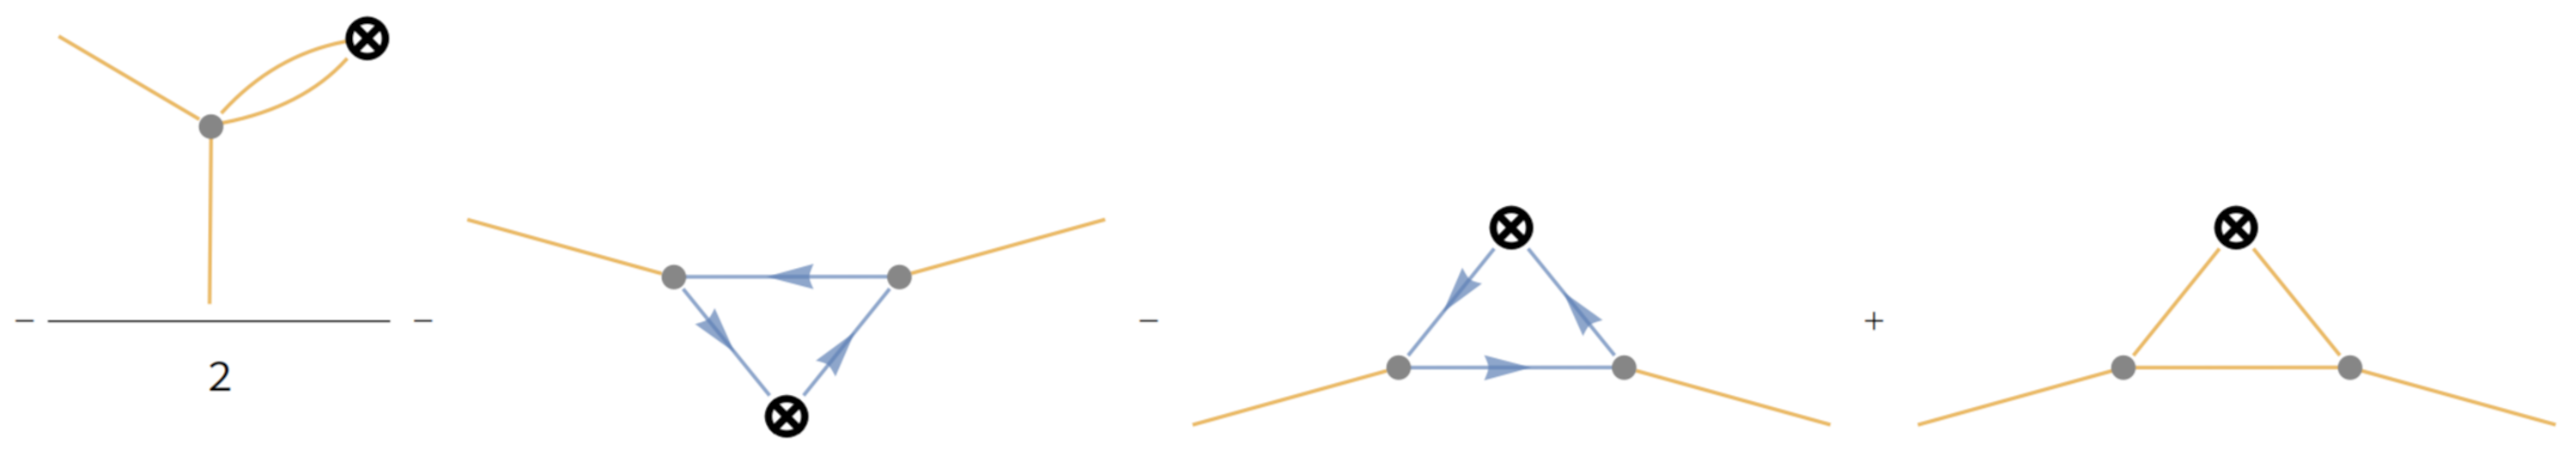
\includegraphics[width=1.05\linewidth]{Mathematica_Gluon2P_3.png}}
\end{equation*}
\end{minipage}
\end{widetext}
%

\subsection{Routing momenta and group indices}

Finally, the superfield indices have to be turned into explicit group indices, and the momenta occurring in diagrams need to be routed, including thus appearing loop momenta.
\FunKit uses the information given through the \mathem{"FieldSpace"} definition in the setup to do both momentum and index routing. This can be immediately done using the \mathem{\mmaDef{FRoute}} function:
%
\begin{widetext}
%\vspace{-2pt}
\hspace{-25pt}
\begin{minipage}{0.8\linewidth}
\begin{mmaCell}{Input}
 \mmaDef{TakeDerivatives}[\mmaDef{setup}, \mmaDef{wEq}, \{A[i1], A[i2]\}]//\mmaDef{FTruncate}//\mmaDef{FRoute}//\mmaDef{FPrint};
\end{mmaCell}
\vspace{-3.0ex}
\begin{equation*}
\put(-159,0){\footnotesize\medmuskip=0mu
	$
	\begin{aligned} &\int_{l_1}(-G_{\bar{c}^{\text{a}}c^{\text{b}}}(l_1,-l_1)\,\Gamma_{c^{\text{b}}\bar{c}^{\text{d}}A^{\text{m}}}(l_1,p_1-l_1,-p_1)\,G_{\bar{c}^{\text{d}}c^{\text{f}}}(l_1-p_1,p_1-l_1)\,\Gamma_{c^{\text{f}}\bar{c}^{\text{h}}A^{\text{n}}}(l_1-p_1,-l_1,p_1)\,G_{\bar{c}^{\text{h}}c^{\text{j}}}(l_1,-l_1)\,\partial_t R_{c^{\text{j}}\bar{c}^{\text{a}}}(l_1,-l_1))
		\\ &\,+\,\int_{l_1}(-G_{\bar{c}^{\text{a}}c^{\text{b}}}(l_1,-l_1)\,\Gamma_{c^{\text{c}}\bar{c}^{\text{a}}A^{\text{m}}}(l_1+p_1,-l_1,-p_1)\,G_{\bar{c}^{\text{e}}c^{\text{c}}}(l_1+p_1,-l_1-p_1)\,\Gamma_{c^{\text{g}}\bar{c}^{\text{e}}A^{\text{n}}}(l_1,-l_1-p_1,p_1)\,G_{\bar{c}^{\text{i}}c^{\text{g}}}(l_1,-l_1)\,\partial_t R_{c^{\text{b}}\bar{c}^{\text{i}}}(l_1,-l_1))
		\\ &\,+\,\int_{l_1}G_{A^{\text{a}}A^{\text{b}}}(-l_1,l_1)\,\Gamma_{A^{\text{m}}A^{\text{c}}A^{\text{b}}}(-p_1,l_1+p_1,-l_1)\,G_{A^{\text{c}}A^{\text{f}}}(-l_1-p_1,l_1+p_1)\,\Gamma_{A^{\text{g}}A^{\text{f}}A^{\text{n}}}(l_1,-l_1-p_1,p_1)\,G_{A^{\text{g}}A^{\text{j}}}(-l_1,l_1)\,\partial_t R_{A^{\text{j}}A^{\text{a}}}(-l_1,l_1)
		\\ &\,+\,\int_{l_1}(-\frac{1}{2}\,G_{A^{\text{a}}A^{\text{b}}}(-l_1,l_1)\,\Gamma_{A^{\text{i}}A^{\text{c}}A^{\text{b}}A^{\text{j}}}(-p_1,l_1,-l_1,p_1)\,G_{A^{\text{c}}A^{\text{f}}}(-l_1,l_1)\,\partial_t R_{A^{\text{f}}A^{\text{a}}}(-l_1,l_1))
	\end{aligned}
	$
}
\end{equation*}
\end{minipage}
\end{widetext}
%
The \mathem{\mmaDef{FRoute}} command groups together terms with the same loop order and additionally provides both the explicit indices of all external momenta and the names of all loop momenta. Explicitly, consider the DSE for the gluon two-point function:
%
\begin{widetext}
%\vspace{-2pt}
\hspace{-30pt}
\begin{minipage}{1.0\linewidth}
\begin{mmaCell}{Input}
 gluonDSE = \mmaDef{TakeDerivatives}[\mmaDef{MakeDSE}[A[i1]], \{A[i2]\}]//\mmaDef{FTruncate}//\mmaDef{FRoute};
 {gluonDSE}["0-Loop"]//\mmaDef{FPrint}
 {gluonDSE}["1-Loop"]["LoopMomenta"]
 {gluonDSE}["1-Loop"]//\mmaDef{FPrint};
 {gluonDSE}["2-Loop"]//\mmaDef{FPlot};
\end{mmaCell}
\vspace{-3.0ex}
\begin{equation*}
\put(-206,0){\footnotesize
	$
	2\,S_{A^{\text{a}}A^{\text{b}}}(-p_1,p_1)
	$
}
\end{equation*}
\vspace{-5.2ex}
\begin{mmaCell}{Output}
 <|"Expression"->FEx[FTerm[2,S[\{A,A\},\{\{-p1,\{v2,c2\}\},\{p1,\{v1,c1\}\}\}]]],
   "ExternalIndices"->\{i1->\{p1,\{v1,c1\}\},i2->\{-p1,\{v2,c2\}\}\},"LoopMomenta"->\{\}|>
\end{mmaCell}
\begin{mmaCell}{Output}
 \{l1\}
\end{mmaCell}
\vspace{-2.0ex}
\begin{equation*}\medmuskip=0mu
	\put(-206,0){\footnotesize
		$
\begin{aligned}
	&\int_{l_1}(-G_{\bar{c}^{\text{a}}c^{\text{b}}}(l_1,-l_1)\,\Gamma_{c^{\text{b}}\bar{c}^{\text{d}}A^{\text{m}}}(l_1,p_1-l_1,-p_1)\,G_{\bar{c}^{\text{d}}c^{\text{f}}}(l_1-p_1,p_1-l_1)\,\Gamma_{c^{\text{f}}\bar{c}^{\text{h}}A^{\text{n}}}(l_1-p_1,-l_1,p_1)\,G_{\bar{c}^{\text{h}}c^{\text{j}}}(l_1,-l_1)\,\partial_t R_{c^{\text{j}}\bar{c}^{\text{a}}}(l_1,-l_1))
	\\ &\,+\,\int_{l_1}(-G_{\bar{c}^{\text{a}}c^{\text{b}}}(l_1,-l_1)\,\Gamma_{c^{\text{c}}\bar{c}^{\text{a}}A^{\text{m}}}(l_1+p_1,-l_1,-p_1)\,G_{\bar{c}^{\text{e}}c^{\text{c}}}(l_1+p_1,-l_1-p_1)\,\Gamma_{c^{\text{g}}\bar{c}^{\text{e}}A^{\text{n}}}(l_1,-l_1-p_1,p_1)\,G_{\bar{c}^{\text{i}}c^{\text{g}}}(l_1,-l_1)\,\partial_t R_{c^{\text{b}}\bar{c}^{\text{i}}}(l_1,-l_1))
	\\ &\,+\,\int_{l_1}G_{A^{\text{a}}A^{\text{b}}}(-l_1,l_1)\,\Gamma_{A^{\text{m}}A^{\text{c}}A^{\text{b}}}(-p_1,l_1+p_1,-l_1)\,G_{A^{\text{c}}A^{\text{f}}}(-l_1-p_1,l_1+p_1)\,\Gamma_{A^{\text{g}}A^{\text{f}}A^{\text{n}}}(l_1,-l_1-p_1,p_1)\,G_{A^{\text{g}}A^{\text{j}}}(-l_1,l_1)\,\partial_t R_{A^{\text{j}}A^{\text{a}}}(-l_1,l_1)
	\\ &\,+\,\int_{l_1}(-\frac{1}{2}\,G_{A^{\text{a}}A^{\text{b}}}(-l_1,l_1)\,\Gamma_{A^{\text{i}}A^{\text{c}}A^{\text{b}}A^{\text{j}}}(-p_1,l_1,-l_1,p_1)\,G_{A^{\text{c}}A^{\text{f}}}(-l_1,l_1)\,\partial_t R_{A^{\text{f}}A^{\text{a}}}(-l_1,l_1))
\end{aligned}
		$
	}
\put(-201,-90){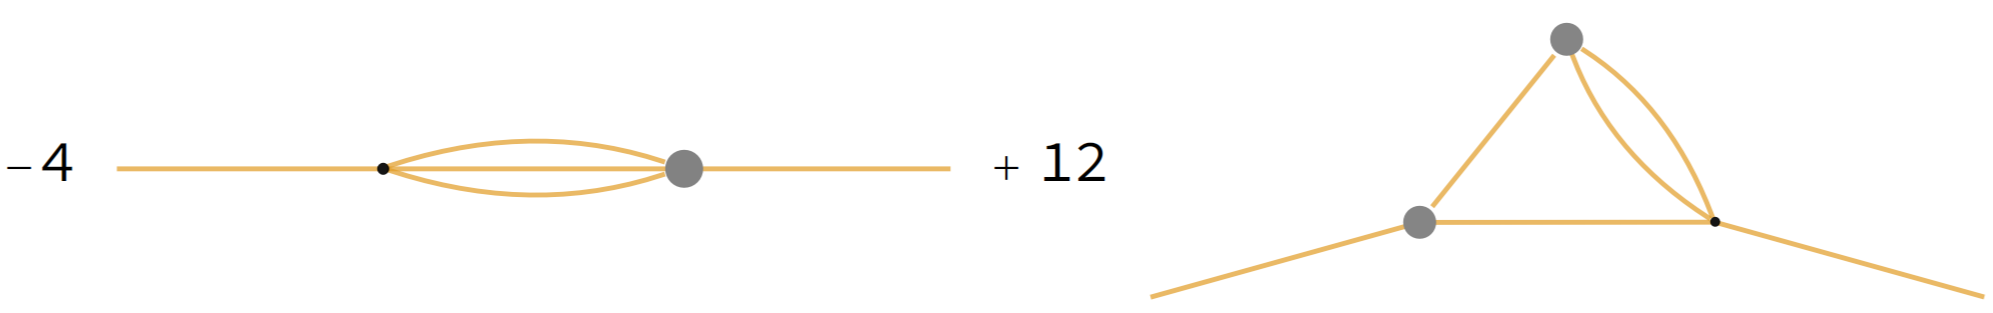
\includegraphics[width=0.5\linewidth]{Mathematica_Gluon2P_4.png}}
\end{equation*}
\end{minipage}
\end{widetext}
%
In the above example, we see also that the command \mathem{\mmaDef{FPrint}} can be inserted during a chain of operations, as it only prints the \LaTeX\xspace output and then returns its argument unchanged.



%%%%%%%%%%%%%%%%%%%%
\subsection{Rules}
\label{sec:FEDeriK_rules}

Internally, to enable a reliable and concise handling of the above features, \FunKit makes abundant use of the superfield notation introduced in \cite{Pawlowski:2005xe}. Especially keeping track of signs for Grassmann fields is ensured by making use of such a notation. Therefore, we briefly introduce the most important points thereof and give a list of the rules used internally in \FEDeriK.

First of all, for the treatment of Grassmann-valued fields, we introduce a field metric, as also in \cite{Pawlowski:2005xe, Braun:2025gvq},
%
\begin{equation}\label{eq:metric}
	\gamma_{ab} = \gamma^{ab} = \begin{cases}
		\begin{pmatrix}
			0 & -1 \\
			1 & 0
		\end{pmatrix}\,\delta_{ab}
		& \text{if $a$ and $b$ are fermionic,} \\[3ex]
		\delta_{ab} & \text{if $a$ and $b$ are bosonic,}   \\[2ex]
		0               & \text{otherwise} 
		\,.
	\end{cases}
\end{equation}
%
This metric can be used to lower and raise indices of arbitrary tensors involving fields. We use the Northwest-Southeast convention to raise and lower indices, i.e.
%
\begin{equation}
	\Phi_a = \Phi^b\gamma_{ba} \,,
	\quad \quad
	\Phi^a = \gamma^{ab}\Phi_b \,.
\end{equation}
%
From the definition of the metric \labelcref{eq:metric}, we can directly infer the commonly found contractions
%
\begin{align}
	\gamma^{a}_{\phantom{a}c} &= \gamma^{ab}\gamma_{bc} = (-1)^{ac}\delta^a_c
	\,,\notag\\[1ex]
	\gamma_{a}^{\phantom{a}c} &= \gamma^{bc}\gamma_{ba} = \delta^a_c
	\,,
\end{align}
%
where we have also introduced
%
\begin{equation}
	(-1)^{ab} = \begin{cases}
		-1 & \text{if both $a$ and $b$ are fermionic,} \\[1ex]
		1 & \text{otherwise} 
		\,.
	\end{cases}
\end{equation}
%
We briefly note that, as a consequence, $\gamma^{a}_{\phantom{a}c}\gamma^{c}_{\phantom{c}d} = \delta^{ad}$.
In \FunKit, $\gamma_{ab}$ is represented\linebreak as \mmaInlineCell{Input}{\mmaDef{\(\pmb{\gamma}\)}[\{\mmaDef{AnyField},\mmaDef{AnyField}\},\{-a,-b\}]}, whereas $(-1)^{ab}$ can be written as \mmaInlineCell{Input}{\mmaDef{FMinus}[\{\mmaDef{AnyField},\mmaDef{AnyField}\},\{a,b\}]}.


Any field derivative in \FEDeriK is directly expressed using the metric, with the full set of rules being
%
\begin{align}
	\frac{\delta \Phi^b}{\delta \Phi^a} &= \gamma_a^{\phantom{a}b}
	\,,\qquad
	\frac{\delta \Phi_b}{\delta \Phi^a} = \gamma_{ab}
	\,,\notag\\[1ex]
	\frac{\delta \Phi_b}{\delta \Phi_a} &= \gamma^{ba}
	\,,\qquad
	\frac{\delta \Phi_b}{\delta \Phi_a} = \gamma^{a}_{\phantom{a}b}
	\,.
\end{align}
%
Similarly, for any correlation function $F$, e.g. the 1PI effective action $F=\Gamma$, 
%
\begin{align}
	\frac{\delta }{\delta \Phi^a} F_{bc\ldots} = F_{abc\ldots}
	\,,\notag\\[1ex]
	\frac{\delta }{\delta \Phi_a} F_{bc\ldots} = F^{a}_{\phantom{a}bc\ldots}
	\,.
\end{align}
%
Specifically for approaches building on the 1PI effective action, we additionally provide the rules for the relation between the propagator $G^{ab} = \frac{\delta^2 W}{\delta J_a \delta J_b}$ and the 1PI two-point function $\Gamma_{ab} = \frac{\delta^2 \Gamma}{\delta \Phi^a \delta \Phi^b}$. 

We derive the relation between these two from the quantum equation of motion, first using left-derivatives,
%
\begin{align}\label{eq:propInvLeft}
	\frac{\delta \Gamma}{\delta \Phi^a} &= \gamma^d_{\phantom{d}a}J_d
	\,,\notag\\[1ex]\Leftrightarrow 
	\frac{\delta \Gamma}{\delta J_b\delta \Phi^a} &= \gamma^b_{\phantom{b}a}
	\,,\notag\\[1ex]\Leftrightarrow 
	\frac{\delta \Phi^c}{\delta J_b}\frac{\delta \Gamma}{\delta \Phi^c\delta \Phi^a} &= \gamma^b_{\phantom{b}a}
	\,,\notag\\[1ex]\Leftrightarrow 
	G^{bc}\Gamma_{ca} &= \gamma^b_{\phantom{b}a}
	\,.
\end{align}
%
and, using right-derivatives,
%
\begin{align}\label{eq:propInvRight}
	\frac{\delta \Gamma}{\delta \Phi^a\delta J_b} &= \gamma_a^{\phantom{a}b}
	\,,\notag\\[1ex]\Leftrightarrow 
	\frac{\delta \Gamma}{\delta \Phi^a\delta \Phi^c}\gamma^c_{\phantom{c}d}\left(\Phi^d\frac{\overset{\leftarrow}{\delta}}{\delta J_b}\right) &= \gamma_a^{\phantom{a}b}
	\,,\notag\\[1ex]\Leftrightarrow 
	\Gamma_{ac}\gamma^c_{\phantom{c}d}G^{db} &= \gamma_a^{\phantom{a}b}
	\,.
\end{align}
%
We can take a derivative $\frac{\delta}{\delta\Phi^f}$ of \labelcref{eq:propInvLeft} and use \labelcref{eq:propInvRight} to obtain the rule
%
\begin{align}
	\left(\frac{\delta}{\delta \Phi^f}G^{ba}\right) 
	&= (-1)(-1)^{bf}(-1)^{dd}\, G^{bc}\Gamma_{cfd}G^{da}\,.
\end{align}
%


%%%%%%%%%%%%%%%%%%%%
\subsection{Teaching FEDeriK}
\label{sec:FEDeriK_teaching}


%%%%%%%%%%%%%%%%%%%%%%%%%%%%%%
\section{Diagrammatic rules and tracing of expressions}
\label{sec:AnSEL}

After having derived the functional equation, it is necessary to use a set of diagrammatic rules to obtain an explicit expression for a given diagram. \FunKit provides functions to automatically create such rules from a chosen set of tensor bases.

To obtain the diagrammatic rules, \FunKit interfaces with the \TensorBases \cite{Braun:2025gvq} package, which provides the tensor expressions for interaction vertices. In \FunKit, a set of vertex bases is specified inside the \mathem{setup}.
%
\begin{mmaCell}{Input}
 bases = <|
   \mmaDef{GammaN}->\{
     \{A,A\}->\{"AA",1\},
     \{A,A,A\}->"AAAClass",
     \{A,A,A,A\}->"AAAAClass",
     \{A,cb,c\}->\{"Acbc",1\},
     \{cb,c\}->"cbc"\},
   \mmaDef{S}->\{
     \{A,A\}->\{"AA",\{1\}\},
     \{A,A,A\}->"AAAClass", 
     \{A,A,A,A\}->"AAAAClass",
     \{A,cb,c\}->\{"Acbc",1\},
     \{cb,c\}->"cbc"\},
   \mmaDef{Propagator}->\{\{A,A\}->"AA",\{cb,c\}->"cbc"\},
   \mmaDef{Rdot}->\{\{A,A\}->\{"AA",1\},\{cb,c\}->"cbc"\}
 |>;
 
 setup = <|
   "FieldSpace" -> \mmaDef{fields},
   "Truncation" -> \mmaDef{truncation},
   "FeynmanRules" -> bases
  |>
\end{mmaCell}
%
In particular, there are three ways to specify vertex bases:
%
\begin{enumerate}[(i)]
	\item Giving only a name, e.g. \mathem{{A,A,A}->"AAAClass"}, which uses the full basis specified as \mathem{"AAAClass"}.
	\item Picking a single element from a larger basis, as in \mathem{{A,cb,c}->{"Acbc",1}}, which uses only the first vertex basis element of \mathem{"Acbc"}.
	\item Picking a subset of a larger basis, e.g. in QCD one could use \mathem{{A,qb,q}->{"AqbqDirect",{1,4,7}}} to pick out the most relevant basis elements 1, 4 and 7 from a standard quark-gluon tensor basis \mathem{"AqbqDirect"}, see \cite{Cyrol:2017ewj, Braun:2025gvq}.
\end{enumerate}
%
with the above definition of \mathem{\mmaDef{setup}}, the diagrammatic rules can be automatically derived using
%
\begin{mmaCell}{Input}
 diagRules = \mmaDef{MakeDiagrammaticRules}[];
\end{mmaCell}
%
With this, one can directly obtain the explicit expressions for diagrams. For example, the 0-loop term of the gluon propagator DSE can be calculated as
%
\begin{mmaCell}{Input}
 DSEAA = \mmaDef{TakeDerivatives}[
   \mmaDef{MakeDSE}[Setup, A[i1]], \{A[i2]\}
  ]//\mmaDef{FTruncate}//\mmaDef{FSimplify}//\mmaDef{FRoute};
 DSEAA["0-Loop"]["Expression"]
 DSEAA["0-Loop"]["Expression"]/.\mmaDef{diagRules}
\end{mmaCell}
%
\begin{mmaCell}{Output}
 FEx[FTerm[2,
   S[\{A,A\},\{\{-p1,\{v2,c2\}\},\{p1,\{v1,c1\}\}\}]]]
\end{mmaCell}
%
\begin{mmaCell}{Output}
 FEx[FTerm[2,deltaAdjCol[c2,c1]
   dressing[S,\{A,A\},1,\{-p1,p1\}]
   transProj[p1,v2,v1]]]
\end{mmaCell}
%
To obtain fully traced expressions, we usually need to use a projector to obtain the coefficient of a single element of the larger tensor basis. For the gluon propagator DSE, we can use the projector included in \TensorBases to 
%
\begin{mmaCell}{Input}
 \mmaDef{FormTrace}[
   \mmaDef{F}[
     \mmaDef{TBGetProjector}["AA",1,\{i1,i2\}/.
       \mmaDef{DSEAA}["1-Loop"]["ExternalIndices"]], \mmaDef{DSEAA}["1-Loop"]["Expression"]/.
       \mmaDef{diagRules}
   ]
 ];
\end{mmaCell}
%
This outputs the 1-loop contributions to the gluon propagator DSE. Similarly, the above calculation can be performed for all diagrams appearing in the DSEs of the Yang-Mills system.

An example, deriving a full set of DSEs and flow equations for Yang-Mills theory with the above specified truncation, can be found in \texttt{examples/Yang-Mills.nb} in the \FunKit repository.

\clearpage
%%%%%%%%%%%%%%%%%%%%%%%%%%%%%%
\section{D\MakeLowercase{i}ANE}
\label{sec:DiANE}

The module \DiANE, \textbf{Di}agram \textbf{A}rts and \textbf{N}otation of \textbf{E}quations, provides visualisation functions for \FunKit. 
\DiANE can both generate publication-ready \LaTeX\xspace code and display equations directly in Mathematica. For example, consider the DSE for the gluon one-point function, given by
%
\begin{equation}
	\Gamma_{A} = \left\langle \frac{\delta S}{\delta A} \right\rangle_{\phi^a = \Phi^a + G^{ab}\frac{\delta}{\delta\Phi^b}}
	\,.
\end{equation}
%
In Mathematica, we can directly derive it and show the rendered \LaTeX\xspace output using
%
\begin{widetext}
\begin{mmaCell}{Input}
 \mmaDef{MakeDSE}[A[x]]//.\{c[_]:>0, cb[_]:>0\}//\mmaDef{FTruncate}//\mmaDef{FSimplify}//\mmaDef{FRoute}//\mmaDef{FPrint}
\end{mmaCell}
%
\vspace{-3.0ex}
\begin{equation*}
	\put(-206,0){\footnotesize
		$
\begin{aligned}&
	\begin{aligned}&
		2\,S_{A^\text{a}A^\text{b}}(0,0)\,A^\text{b}(0)
		\\ &\,+\,
		3\,S_{A^\text{a}A^\text{b}A^\text{c}}(0,0,0)\,A^\text{b}(0)\,A^\text{c}(0)
		\\ &\,+\,
		4\,S_{A^\text{a}A^\text{b}A^\text{c}A^\text{d}}(0,0,0,0)\,A^\text{b}(0)\,A^\text{c}(0)\,A^\text{d}(0)
	\end{aligned}
	\\&
	\begin{aligned}&
		\,+\,    \int_{l_1}3\,S_{A^\text{e}A^\text{a}A^\text{b}}(0,l_1,-l_1)\,G_{A^\text{b}A^\text{a}}(l_1,-l_1)
		\\ &\,+\,
		\int_{l_1}12\,S_{A^\text{e}A^\text{a}A^\text{f}A^\text{b}}(0,l_1,0,-l_1)\,A^\text{f}(0)\,G_{A^\text{b}A^\text{a}}(l_1,-l_1)
		\\ &\,+\,
		\int_{l_1}(-S_{c^\text{a}\bar{c}^\text{b}A^\text{e}}(l_1,-l_1,0)\,G_{\bar{c}^\text{b}c^\text{a}}(l_1,-l_1))
	\end{aligned}
	\\&
	\,+\,\int_{l_1}\int_{l_2}(-4\,S_{A^\text{m}A^\text{g}A^\text{a}A^\text{e}}(0,l_2,l_1,-l_1-l_2)\,G_{A^\text{a}A^\text{b}}(-l_1,l_1)\,G_{A^\text{e}A^\text{f}}(l_1+l_2,
	-l_1-l_2)\,\Gamma_{A^\text{f}A^\text{b}A^\text{h}}(l_1+l_2,-l_1,-l_2)\,G_{A^\text{h}A^\text{g}}(l_2,-l_2))
\end{aligned}
		$
	}
\end{equation*}
\end{widetext}

The typesetting code for the above equation can be also read out using the \mathem{\mmaDef{FTex}} command, and copied over to a document. Internally, we use \texttt{MaTeX} \cite{szabolcs_horvat_2024_10828124} to render the \LaTeX\xspace code inside Mathematica. This requires the \bash{pdflatex} command to be available on the system.

Nota that we have already used the \mathem{\mmaDef{FPrint}} and \mathem{\mmaDef{FPlot}} commands in the previous sections to showcase the results of our computations.


%%%%%%%%%%%%%%%%%%%%%%%%%%%%%%
\section{Automatic Code Generation}
\label{sec:COEN}

\FunKit provides a set of tools to conveniently translate the Mathematica expressions resulting after performing all traces into code that can be directly incorporated into a numerical program.
To that end, \FunKit provides direct output to Fortran and Julia functions, and a set of functions to generate C++ classes and methods with arbitrary types by means of templates.
%
\begin{widetext}
%
\begin{mmaCell}{Input}
 MakeJuliaFunction[
   DSEAAResult["1-Loop"] /. cos[p, l1] -> cospl1,
   "Parameters" -> {"l1", "cos", "p", "gS", "ZA", "Zc", "ZA3", "ZAcbc", 
     "ZA4"},
   "Name" -> "DSE_kernel_AA_1Loop",
   "Body" -> "cospl1 = cos"
  ]
\end{mmaCell}
%
\begin{mmaCell}{Output}
 function DSE_kernel_AA_1Loop(l1, cos, p, gS, ZA, Zc, ZA3, ZAcbc, ZA4)
   cospl1 = cos
   _repl1 = Zc(l1)
   _repl2 = Zc(sqrt(l1^2 + 2*cospl1*l1*p + p^2))
   return gS*(24*gS*(2 + cospl1^2*(1 - 1/(_repl1*l1^2)) + 7/(_repl1*l1^2)) - (3*(4*cospl1^4*l1^2*(-1 + _repl1*l1^2)*p^2 + _repl1*(2*l1^6 + 3*l1^4*p^2 + _repl2*l1^2*p^4*(l1^2 + p^2)) + 2*(6*l1^4 + 16*l1^2*p^2 + 6*p^4 + _repl2*(l1^2 - p^2)^2*(l1^2 + p^2)) + 2*cospl1*l1*p*(2*_repl2*(l1^2 - p^2)^2 + 12*(l1^2 + p^2) + _repl1*l1^2*(7*l1^2 + 6*p^2 + _repl2*p^4)) + cospl1^2*(_repl2*(l1^2 - p^2)^2*(l1^2 + p^2) - 4*(3*l1^4 + 7*l1^2*p^2 + 3*p^4) + _repl1*l1^2*(l1^4 + 32*l1^2*p^2 + 12*p^4 - _repl2*p^4*(l1^2 + p^2))) + 2*cospl1^3*l1*p*(_repl2*(l1^2 - p^2)^2 - 12*(l1^2 + p^2) + _repl1*l1^2*(-(_repl2*p^4) + 2*(l1^2 + 6*p^2))))*ZA3(sqrt(0.6666666666666666)*sqrt(l1^2 + cospl1*l1*p + p^2)))/(_repl1*_repl2*l1^2*(l1^2 + 2*cospl1*l1*p + p^2)^2) + ((-1 + cospl1^2)*ZccbA(sqrt(0.6666666666666666)*sqrt(l1^2 + cospl1*l1*p + p^2)))/((l1^2 + 2*cospl1*l1*p + p^2)*ZA(l1)*ZA(sqrt(l1^2 + 2*cospl1*l1*p + p^2))))
 end
\end{mmaCell}
%
\end{widetext}


%%%%%%%%%%%%%%%%%%%%
\begin{acknowledgments}
We thank... for discussions. This work is done within the fQCD collaboration \cite{fQCD} and we thank its members for discussions and collaborations on related projects.
FRS acknowledges funding by the GSI Helmholtzzentrum f\"ur Schwerionenforschung and by HGS-HIRe for FAIR.

This work is funded by the Deutsche Forschungsgemeinschaft (DFG, German Research Foundation) under Germany’s Excellence Strategy EXC 2181/1 - 390900948 (the Heidelberg STRUCTURES Excellence Cluster) and the Collaborative Research Centre SFB 1225 (ISOQUANT). It is also supported by EMMI. 
	
	
\end{acknowledgments}

%%%%%%%%%%%%%%%%%%%%
\appendix


%%%%%%%%%%%%%%%%%%%%
\section{Notation}
\label{app:notation}

In the following, we briefly detail our notation for describing tensor bases of general QFTs.
To keep the notation concise and general, we collect all fields of the theory at hand into a single superfield~$\Phi$. 
We do this for all general arguments but make fields and indices explicit for specific examples.
Furthermore, we absorb all indices of the superfield, including momenta and group indices, into a single general multi-index.

An index~$a$ for a field~$\Phi^a$ contains momentum and possibly Lorentz, colour, flavour or further indices of the corresponding field.
Wherever indices are explicitly given, we use Greek letters~$\mu$,~$\nu$,~$\rho$,~$\sigma$,~$\dotsc$ for Lorentz indices and Latin letters~$a$,~$b$,~$c$,~$\dotsc$ for indices associated with any other type of group. 

While for bosons no additional structure needs to be imposed on the superfield, it is necessary to take into account that fermion and anti-fermion fields always come in pairs.
To that end, we use the field-space metric given by
%
\begin{equation}
	\gamma_{ab} = \gamma^{ab} = \begin{cases}
		\begin{pmatrix}
			0 & -1 \\
			1 & 0
		\end{pmatrix}\,\delta_{ab}
		& \text{if $a$ and $b$ are fermionic,} \\[3ex]
		\delta_{ab} & \text{if $a$ and $b$ are bosonic,}   \\[2ex]
		0               & \text{otherwise} 
		\,.
	\end{cases}
\end{equation}
%
One can now raise and lower indices of a super-field using the metric
%
\begin{equation}
	\Phi_a = \Phi^b\gamma_{ba} \,,
	\quad \quad
	\Phi^a = \gamma^{ab}\Phi_b \,.
\end{equation}
%
Raising and lowering indices, as introduced at the example of the superfield (vector), also applies to general higher rank tensors, e.g.
%
\begin{equation}
	M^{ab}_{\phantom{ab}c} = \gamma^{aa'} \gamma^{bb'} M_{a'b'}^{\phantom{a'b'}c'} \gamma_{c'c}
	\,.
\end{equation}
%
With this, derivatives of an arbitrary functional~$F[\Phi]$ are written as
%
\begin{equation}
	F_{a_1 a_2 \ldots a_n}[\Phi] =
	\frac{\delta}{\delta \Phi^{a_1}} \frac{\delta}{\delta \Phi^{a_2}} \ldots \frac{\delta}{\delta \Phi^{a_n}} F[\Phi]
	\,.
	\label{eq:Falpha}
\end{equation}
%
For convenience, we always consider all momenta to be incoming, which also fixes our Fourier convention:
%
\begin{equation}
	\Phi^a(x) = \int \frac{d^d p}{(2\pi)^d} e^{ipx}\Phi^a(p)
	\,.
\end{equation}
%	
Finally, we write the general decomposition of an~$n$-th derivative of~$F[\Phi]$ as
%
\begin{equation}\label{eq:general_decomposition}
	F_{\alpha}[\Phi] = (2\pi)^d\ \delta^{(d)}\left( \sum_{i=1}^n p_i \right)\,
	\sum_{i=1}^{N_\alpha} \tau_{i,\alpha} \, \lambda_{i,\alpha}
	\,,
\end{equation}
%
where we have employed an even more compact notation by introducing the multi-index~$\alpha = (a_1, a_2, \ldots, a_n)$. 
This index includes all field indices.
Here, the~$\{\tau_{i,\alpha}\}$ are some basis of dimension~$N_\alpha$ of the tensor space of the Green's function, while the~$\{\lambda_{i,\alpha}\}$ are the coefficients of the expansion of~$F^\alpha$ within this basis.

Note that no summation over $\alpha$ is implied in \labelcref{eq:general_decomposition}: the basis elements may fully depend on the elements of the multi-index $\alpha$, whereas the coefficients depend at least on the momenta of the particles  contained in $\alpha$.
If additional ``continuous indices" are present, these can also be included as dependences of the dressings. 

For example, in \labelcref{eq:general_decomposition} the coefficients~$\lambda_i$ can be chosen such that they have an additional field dependence, e.g. coming from some composite operator $\phi[\Phi]$, which is useful if the associated symmetry is spontaneously broken. 
An example would be the composite field $\phi[\Phi] = \bar q q$ in QCD, which obtains a finite expectation value in the vacuum.
Any such rewriting either changes~$N_\alpha$ from uncountable infinity to a finite number, or, as in the above example, changes the expansion point of the interaction (i.e. the field background).

Furthermore, note that if~$F[\Phi] = \Gamma[\Phi]$, we call~$\Gamma_\alpha[\Phi]$ a \textit{vertex} of the theory and~$\{\lambda_i\}$ are the corresponding \textit{dressings}.

\newpage
%%%%%%%%%%%%%%%%%%%%
\bibliography{bibliography}
%%%%%%%%%%%%%%%%%%%%

\end{document}